В данной работе для изучения микролинзирования используется вычислительная программа {\tt{microlens}} (\cite{wambsganss1992-microlens}, \cite{wambsganss1999}), которая моделирует методом обратной трассировки лучей (\textit{inverse ray shooting}) распределение каустик в плоскости источника, основываясь на распределении звёзд в плоскости линзы. Выходными данными этой программы являются карты микрокаустик - двумерные массивы (с координатами пикселей), содержащие значения обусловленного микролинзированием усиления в плоскости источника. Основными параметрами для каждой карты являются безразмерные поверхностные плотности звёзд $\kappa_*$ и непрерывно распределенной тёмной материи $\kappa_c$ (либо параметр $s=\kappa_c/(\kappa_*+\kappa_c)$) в линзирующей галактике, внешний сдвиг $\gamma$, учитывающий вклад гравитационного потенциала скопления галактик, а также функция масс звёзд. 

%Dobler, Keeton 2006

%Several authors have shown that microlensing magnification distributions are insensitive to the mean mass ¯m (Wyithe & Turner 2001; Schechter et al. 2004; Mortonson et al. 2004). For microlensing of SN light curves, the mean mass does set an overall time scale: as ¯m increases, the time it takes for the source to reach a given fraction of R¯ scales as ¯m1/2

%The properties of the microlensing fluctuations should be dependent on the stellar population parameters (namely f∗ and q). They also depend on the particular configuration of stars, because as shown in Figure 2 different realizations of stellar populations that are statistically equivalent yield very different magnification maps in the source plane. Note that these magnification maps are 2.5R¯ on a side, so a SN will expand to cover roughly half of a map during its observable lifetime.

Здесь и далее для простоты предполагается, что все звезды в галактике имеют одинаковую массу, которая равна массе Солнца $M_{\odot}$. По данным некоторых  исследований эффект микролинзирования слабо зависит от начальной функции масс (каких? \cite{hubersuyu2019}, либо \cite{goldstein2018} секция 3, но только для SN Ia).


Я не помню, одинаковые ли или нет параметры у этих карт. В целом пример можно убрать.

На Рисунке \ref{fig:micromaps} приведены примеры результатов выполнения программы {\tt{microlens}} - карты усилений для двух различных значений количества звёзд, вызывающих микролинзирование. Светлые области означают, что источник усиливается, находясь в них, тёмные - что ослабляется. Видно, что а) сеть каустик намного богаче при большем количестве звёзд-линз, б) по всей карте усиление меняется и почти нигде не остаётся таким, каким его предсказывает модель линзы, то есть в отсутствие микролинзирования.

\begin{figure}[H]
    \centering
	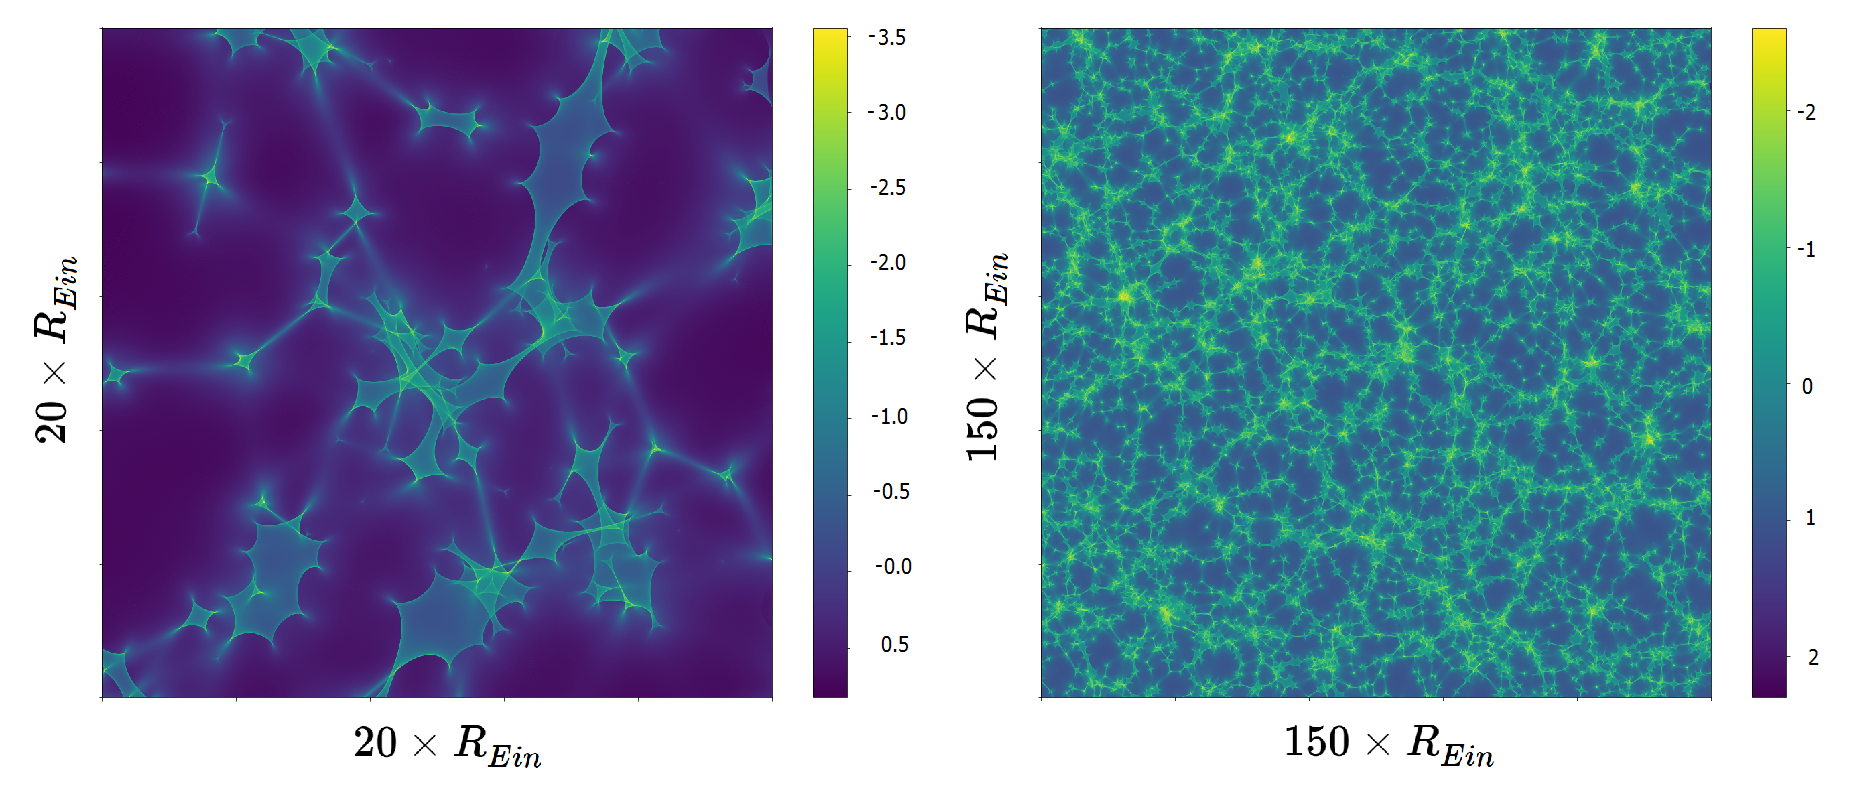
\includegraphics[scale=0.22]{pics/maps_example.png}
	\caption{Карты микрокаустик. Количество звёзд-линз слева - 313, справа - 14526. Цветовая шкала (в единицах звёздных величин) показывает, как дополнительно увеличивается или ослабляется яркость источника вследствие только микролинзирования. \label{fig:micromaps}} 
\end{figure}